% this is source code for one of the sessions in Digital Skills for Research Workshop (EMTTI, University of Wolverhampton)
% March 2022, Maria Kunilovskaya (mkunilovskaya@gmail.com)

\documentclass[a4paper,11pt]{article}

\usepackage[utf8]{inputenc}

\usepackage{geometry}
\geometry{
	a4paper,
	total={170mm,257mm},
	left=20mm,
	top=15mm,
}
\setlength\parindent{0pt} % set all indents to 0

\usepackage{tcolorbox}
\usepackage{listings}  % a verbatim environment which can break lines unlike \verb||
\usepackage{multicol} % allows columns environment

\usepackage{blindtext}
\usepackage{float} % allows \begin{table}[H] for placing tables exactly where you want them

\usepackage[colorlinks=true, linkcolor=blue]{hyperref} % show linky content in blue instead of coloured boxes

%--------------------
% Packages for additional or modified environments
% -------------------
\usepackage{enumerate} % for advanced enumeration: \begin{enumerate}[a)], [i], [1.], [A], [I)], [1)]


%--------------------
% Packages to work with tables
% -------------------
\usepackage{tabularx} % adjusts the table to width adding space to columns set to X
\usepackage{booktabs} % provides the \toprule, \midrule and \bottomrule, \cmidrule for tables
\usepackage{longtable}  % allows a table span across several pages
\usepackage{multirow} % merge rows in a table

%--------------------
% Packages to work with pictures and figures
% -------------------
\usepackage{graphicx}  % to add graphics
\graphicspath{{images/}{pics/}}  % folders with .png, .jpj, .gif, .eps, .pdf
\usepackage{wrapfig} % put figure inside the text
\usepackage{caption} % automatic names for graphics; default Figure
\captionsetup{labelsep=period} % add a dot after Figure in captions

\usepackage{tikz} 
\usetikzlibrary{calc, positioning, shapes.arrows} % allows to set arrow parameters where you need it

\title{Session 3. Tables and figures}
\author{Digital Skills for Research}
\date{March 09, 2022}

\begin{document}

%remove numbering from the first page
\clearpage
\maketitle
\thispagestyle{empty}

\tableofcontents

\section{Environments}

\subsection{LISTs!}

Three predefined types of list environments: \verb|\begin{itemize}, \begin{enumerate}, \begin{description}|

\begin{itemize}
	\item simple bullets
	\item enumerated items (customisable with \verb|\begin{enumerate}[a)], [i], [1.], [A], [I)], [1)]| after importing \verb|\usepackage{enumerate}|)
	\item \verb|\begin{description}| use a list of terms as items and their definitions as values against each item (see an example of~\hypertarget{wd:descr}{description-style list} below)
\end{itemize}

\subsection{Examples of other default environments}

\verb|\begin{center} ... \end{center}|

\begin{center}https://tinyurl.com/yf8orxog
CENTRED TEXT\\
\textbf{Environments are used to apply formatting to blocks of text.}
\end{center}

\verb|\begin{quote}| for short quotes separated by blank lines and \verb|\begin{quotation}| for several indented paragraphs. See \verb|\begin{quote}|:

\begin{quote}
	\lq\lq Don't worry about a thing,\\
	'Cause every little thing gonna be all right.\rq\rq
\end{quote}

\subsection{Examples of imported environments}


\begin{verbatim}

==
This is a demo of an environment \begin{comment}. 
It requires \usepackage{comment} in the preamble. 
Text between == is printed inside \begin{verbatim} environment.

	\begin{comment}
	This is great for multi-line comments 
	such as this one.
	It require \usepackage{comment} in the preamble.
	\end{comment}
==
\end{verbatim}

\verb|\usepackage{multicols}| \\
\verb|\begin{multicols}{3} ... \columnbreak ... \end{multicols}|

\begin{multicols}{3} %remove numbering from the first page
	\clearpage\maketitle
	\thispagestyle{empty}
	
	In Section~\ref{sec:tabs} we will look at some principles of arranging tables.
	\usetikzlibrary{calc, positioning, shapes.arrows}
	\columnbreak 
	This is source code for a basic table:
	\begin{verbatim}
		\begin{tabular}{ c c c } 
		cell1 & cell2 & cell3 \\ 
		cell4 & cell5 & cell6 \\ 
		cell7 & cell8 & cell9 \\ 
		\end{tabular}%\usepackage{pgfplots}
		%\usepackage{pgfplotstable}
	\end{verbatim}

	
	\columnbreak
	This is how it compiles:
	\begin{tabular}{ c c c } 
		cell1 & cell2 & cell3 \\ \usetikzlibrary{calc, positioning, shapes.arrows}
		cell4 & cell5 & cell6 \\ 
		cell7 & cell8 & cell9 \\ 
	\end{tabular}
	\setlength\fboxsep{3pt} % add a frame around a figure and set its distance from content
	\setlength\fboxrule{1pt} % line width for the frame \fbox{}
\end{multicols}

\section{A special case: Tables}\label{sec:tabs}

See Wizards and Latex tabs in your \TeX editor!

\subsection{Basic commands for tables formatting}
\begin{enumerate}[A)]
	\item horisontal lines with \verb|\hline|
	\item vertical lines are lines in c%\usepackage{pgfplots}
	%\usepackage{pgfplotstable}all parameters: \verb-\begin{tabular}{l|c|r|}-;\\ this is NO lines: \verb-\begin{tabular}{ccc}-
	\item \& is a column separator in code
	\item each row ends with \verb|\\|
\end{enumerate}

\medskip

\subsection{Table environments and wizards}

There are several environments to format tables (below is an example of a \hyperlink{wd:desc}{description-style list} mentioned above, and it is a hyperlink to a specific word in the text above; see the source file at GitHub to see how it is coded):
\setlength\fboxsep{3pt} % add a frame around a figure and set its distance from content
\setlength\fboxrule{1pt} % line width for the frame \fbox{}
\begin{description}
	\item[tabular] basic format to stack text horizontally and vertically; is placed as-is in the text, at the position where coded; the width of each column is set with \verb-\begin{tabular}{p{4cm}|c|p{5cm}|}-; even columns with various text placement (left, centre, right): \verb-\begin{tabular}{l|c|r|}-
	\item[table] a float object tha\usetikzlibrary{calc, positioning, shapes.arrows}t determines best position in text; it can contain virtually anything, but often used to wrap \verb|\begin{tabular}|
	\item[tabularx] uses X columns to fit the table to the specified width (\verb-{\begin{tabular}{\textwidth}{X|c|X}-)
	\item[longtable] imported with \verb|\usepackage{longtable}|; codes tables that span across the page boundary

\end{description}

This code generates Table \ref{tab:mytab}.

\begin{lstlisting}[breaklines]
\begin{table}[H] % H Places the float at precisely the location in the LATEX code. Requires the float package.
	\begin{center}
		\caption[Table 1 name for List of Tables]{This table does not make much sense; it is created for demonstration only}\label{tab:mytab}
		\begin{tabular}{|c|c|c|c||l|c|c|r|c|c|}
			\hline
			1 & 2 & 3 & 4 & 5 & 6 & 7 & 8 & 9 & 10 \\ \hline
			first & second & \multicolumn{3}{|c|}{third -- fifth} &   &  & eight &   &  \\ 
			\cline{1-7} \cline{9-10}%\usepackage{pgfplots}
			%\usepackage{pgfplotstable}
			1 & 2 & 3 & 4 & 5 & 6 & 7 & 8 & 9 & 10 \\ \hline
			1 & 2 & 3 & 4 & 5 & 6 & 7 & 8 & 9 & 10 \\ \hline
			\multirow{3}{*}{three rows}  & 2 & 3 & 4 & 5 & 6 & 7 & 8 & 9 & 10 \\ \cline{2-10}
			& 2 & 3 & 4 & 5 & 6 & 7 & 8 & 9 & 10 \\ %\cline{2-10}
			& 2 & 3 & 4 & 5 & 6 & 7 & 8 & 9 & 10 \\ \hline
		\end{tabular}
	\end{center}
	%\caption{You can place the caption below the table}
\end{table}
\end{lstlisting}

\begin{table}[H] % H Places the float at precisely the location in the LATEX code. Requires the float package.
	\begin{center}
		\caption[Table 1 name for List of Tables]{This floating table does not make much sense; it is created for demonstration only}\label{tab:mytab}
		\begin{tabular}{|c|c|c|c||l|c|c|r|c|c|}
			\hline\setlength\fboxsep{3pt} % add a frame around a figure and set its distance from content
			\setlength\fboxrule{1pt} % line width for the frame \fbox{}
			1 & 2 & 3 & 4 & 5 & 6 & 7 & 8 & 9 & 10 \\ \hline
			first & second & \multicolumn{3}{|c|}{third -- fifth} &   &  & eight &   &  \\ 
			\cline{1-7} \cline{9-10}
			1 & 2 & 3 & 4 & 5 & 6 & 7 & 8 & 9 & 10 \\ \hline
			1 & 2 & 3 & 4 & 5 & 6 & 7 & 8 & 9 & 10 \\ \hline
			\multirow{3}{*}{three rows}  & 2 & 3 & 4 & 5 & 6 & 7 & 8 & 9 & 10 \\ \cline{2-10}
			& 2 & 3 & 4 & 5 & 6 & 7 & 8 & 9 & 10 \\ %\cline{2-10}
			& 2 & 3 & 4 & 5 & 6 & 7 & 8 & 9 & 10 \\ \hline
		\end{tabular}
	\end{center}
	% \caption{You can place the caption below the table}
\end{table}

\section{Graphics and drawing}
\subsection{Simple commands}

\textbf{(for raster (.png, .jpg) or vector (.eps) graphics)}

\bigskip
	%\usepackage{pgfplots}
	%\usepackage{pgfplotstable}
Use scaling: \verb|\includegraphics[scale=.2]{raster-vs-vectors.jpg}| \\
\includegraphics[scale=.2]{raster-vs-vectors.jpg}  

\bigskip

Use size (and a frame around the graphics): \verb|	\fbox{\includegraphics[width=50mm]{lines.eps}}| \\
Notice how you can change \verb|\fbox{}| parameters inside the main code:
\verb|\setlength\fboxsep{10pt}| \\

\setlength\fboxsep{10pt} % set its distance of the frame \fbox{} from the content
\setlength\fboxrule{.5pt} % line width for the frame \fbox{}
 	
\fbox{\includegraphics[width=50mm]{lines.eps}}
 
\subsection{Figure environment}
\begin{lstlisting}[breaklines]
\begin{figure}[h] % htbp - position preferences (here, top, bottom, page)
	\includegraphics[scale=1]{cup}
	\caption{Publisher's logo}
	\label{fig:logo}
\end{figure}
\end{lstlisting}

\begin{figure}[h] % htbp

		\centering
		
		\setlength\fboxsep{5pt}\title{Session 3. Tahttps://tinyurl.com/yf8orxogbles and figures}
		\author{Digital Skills for Research}
		\date{\today}
		
		% set its distance of the frame \fbox{} from the content
		\setlength\fboxrule{.2pt} % line width for the frame \fbox{}
			\fbox{\includegraphics[scale=1]{cup}}
		\caption{Publisher's logo}
		\label{fig:logo}
	\usetikzlibrary{calc, positioning, shapes.arrows}
\end{figure}

%\fbox{\textcolor{red}{\rule{1cm}{1cm}}}

Use \verb|\begin{wrapfigure}{r}{0.3333\linewidth}| to use Figures inline (wrapped with the text). For example: \\

\begin{wrapfigure}{r}{0.3333\linewidth}
	\includegraphics[scale=.5]{rasterVSvector.png}
	\caption{Two types of graphics}
	\label{fig:types}
\end{wrapfigure}

Vector graphics are also known as scalable vector graphics (SVG). These graphics consist of anchored dots and connected by lines and curves, similar to the connect-the-dot activities you may have done as a kid. Because these graphics are not based on pixels, they are known as resolution independent, which makes them infinitely scalable. Their lines are sharp, without any loss in quality or detail, no matter what their size. These graphics are also device-independent, which means their quality doesn't depend on the number of dots available on a printer or the number of pixels on a screen. Because they consist of lines and anchor points, the size of the files are relatively small.

You can also use an online \href{https://www.tablesgenerator.com/}{Tables Generator}.

\subsection{Drawing with \href{https://www.overleaf.com/learn/latex/TikZ_package}{TikZ}}

TikZ is the most complex and powerful tool to create vector graphics.
The graphics are put in \verb|\begin{tikzpicture}| environment.

\medskip

To help with calculating coordinates, draw the support grid: \\ \verb|\draw[style=help lines] (-2,0) grid[step=1cm] (8,4);|

\medskip

For each shape there are some drawing instructions. 
For example, 
\begin{itemize}
	\item for a rectangular you have to provide two points, the first one is where the ``pencil'' begins to draw the rectangle and the second one is the diagonally opposite corner point
\end{itemize}

\begin{lstlisting}
\begin{tikzpicture}
	\draw[style=help lines] (-2,0) grid[step=1cm] (8,4);
	\draw (0,0) -- (1,1);
	\draw[red, thick] (-2,0) -- (0,3);
	\draw[blue, very thick] (-1,1) rectangle (2,2);
	\filldraw[color=red!60, fill=red!5, very thick](4,3) circle (1);
	
	% define a style of some object, e.g. an arrow
	\tikzstyle{my arrow} = [draw=brown!75, very thick, single arrow, minimum height=3cm, shape border rotate =#1, fill=brown!10]
	\node at (6,2) [my arrow=90] {\rotatebox{90}{some tendency}};
\end{tikzpicture}
\end{lstlisting}

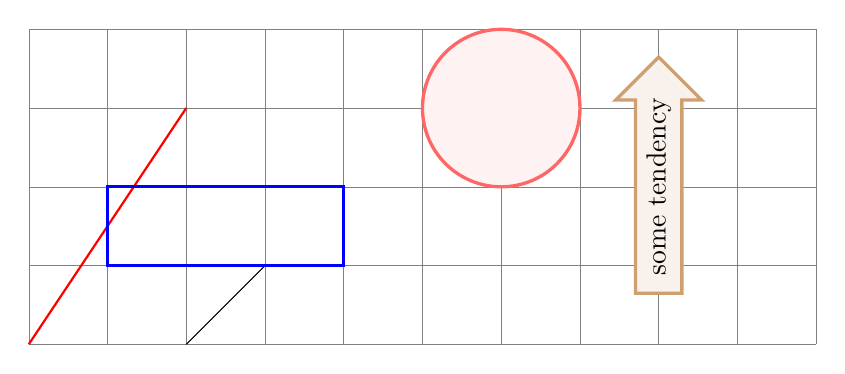
\begin{tikzpicture}
	\draw[style=help lines] (-2,0) grid[step=1cm] (8,4);
	\draw (0,0) -- (1,1);
	\draw[red, thick] (-2,0) -- (0,3);
	\draw[blue, very thick] (-1,1) rectangle (2,2);
	\filldraw[color=red!60, fill=red!5, very thick](4,3) circle (1);
	
	% define a style of some object, e.g. an arrow
	\tikzstyle{my arrow} = [draw=brown!75, very thick, single arrow, minimum height=3cm, shape border rotate =#1, fill=brown!10]
	\node at (6,2) [my arrow=90] {\rotatebox{90}{some tendency}};
\end{tikzpicture}

NB! It might be easier to draw in Python, inc. saving as .eps

\subsection{Produce automatic lists of labelled objects}

\verb|\listoftables and \listoffigures|

\listoftables
\listoffigures

\section*{Task 3. Time-table your pastimes/classes and add pics/graphs}
\label{task}
\addcontentsline{toc}{section}{Task 3.}

\begin{tcolorbox}[width=\textwidth, colback={yellow!40!white}, title={}, colbacktitle=yellow!60!white, coltitle=black]
	\begin{itemize}
		\item Produce a one-page document with a table and a figure. 
		\begin{itemize}
			\item Make a timetable your pastimes/classes or reproduce a table that compares vector and raster images \href{https://tinyurl.com/yf8orxog}{here}, for example
			\item no pagination, please!
			\item add in-text references to both
			\item create proper captions: Chicago referencing style (as required by Benjamins Publishing house) requires ``Figure captions should be placed below the figure, while table captions should be placed above the relevant table.''
			\item demonstrate any other efforts to learn about formatting tables and producing graphics 
		\end{itemize} 
	\end{itemize}
	
\end{tcolorbox}%

\end{document}